\documentclass[12pt, twoside]{article}
\usepackage[letterpaper, margin=1in, headsep=0.5in]{geometry}
\usepackage[english]{babel}
\usepackage[utf8]{inputenc}
\usepackage{amsmath}
\usepackage{amsfonts}
\usepackage{amssymb}
\usepackage{tikz}
\usepackage{yhmath}
\usetikzlibrary{quotes, angles}
\usepackage{graphicx}
\usepackage{enumitem}
\usepackage{multicol}

\newif\ifmeta
\metatrue %print standards and topics tags

\title{Regents Geometry}
\author{Chris Huson}
\date{May 2022}

\usepackage{fancyhdr}
\pagestyle{fancy}
\fancyhf{}
\renewcommand{\headrulewidth}{0pt} % disable the underline of the header
\raggedbottom

\fancyhead[LE]{\thepage}
\fancyhead[RO]{\thepage \\ Name: \hspace{4cm} \,\\}
\fancyhead[LO]{BECA / Dr. Huson / Geometry\\* Unit 11: Function transformations\\* 20 May 2022}

\begin{document}
\subsubsection*{11.17 Quiz: Function transformations}
\begin{enumerate}
\item The standard form of a linear equation is $ax+by=c$, where $x$ and $y$ are variables and $a$, $b$, and $c$ are parameters (fixed numbers).\\[0.25cm]
For example if the equation of a line is $3x+2y=5$, write down the value of each parameter.
  \begin{enumerate}
    \item $a=$
    \vspace{0.5cm}
    \item $b=$
    \vspace{0.5cm}
    \item $c=$
  \end{enumerate} \vspace{0.2cm}

\item The slope-intercept form of a linear equation is $y=mx+b$. The parameter $m$ quantifies the slope and $b$ the $y$-intercept.\\[0.25cm]
For the equation $y=\frac{1}{2}x-7$, write down the value of each parameter..
  \begin{enumerate}
    \item $m=$
    \vspace{0.5cm}
    \item $b=$
    \vspace{0.2cm}
  \end{enumerate}

\item The point-slope form of a linear equation is $y-k=m(x-h)$. Again, the parameter $m$ represents the slope. The parameters $h$ the $h$ are the coordinates of a point that the line passes through.\\[0.25cm]
For the equation $y-3=-\frac{3}{5}(x-7)$, write down the value of each parameter..
  \begin{enumerate}
    \item $m=$
    \vspace{0.5cm}
    \item $h=$
    \vspace{0.5cm}
    \item $k=$
    \vspace{0.5cm}
    \item Write down a point that the line passes through as a coordinate pair.
  \end{enumerate}
  
\item Rewrite each equation in the required form.
  \begin{enumerate}
    \begin{multicols}{2}
      \item   $y=5x-3$ in the form $ax+by=c$
      \item   $y+3=2(x+1)$ in the form $y=mx+b$ 
    \end{multicols}
  \end{enumerate} \vspace{0.5cm}

\newpage
\item   
 \begin{enumerate}
  \item Find the slope $m$ of the line $2x+4y=12$.
  \vspace{2cm}
  \item Write down the slope perpendicular to the line, $m_{\perp}$.
  \vspace{0.5cm}
\end{enumerate}

\item Write down the slope perpendicular to the given slope.
\begin{enumerate}
  \begin{multicols}{2}
    \item   $m= \frac{1}{2} \hspace{1cm} m_{\perp} = $
    \item   $m= -6 \hspace{1cm} m_{\perp} = $ 
  \end{multicols}
\end{enumerate} \vspace{0.5cm}

\item Write down the equation of the line through $(1,-3)$ with a slope of $4$.
\vspace{2cm}

\item The line segment $\overline{AB}$, $A(2,1)$ and $B(8,3)$, is shown below.
  \begin{multicols}{2}
    \begin{enumerate}
    \item Mark the midpoint $M$ of $\overline{AB}$. Label it as an ordered pair.
    \item Find the slope of $\overline{AB}$. \vspace{2cm}
    \item Write down the slope perpendicular to $\overline{AB}$. \vspace{1cm}
    \item Write down the equation of the perpendicular bisector of $\overline{AB}$. \vspace{2cm}
    \item Draw the perpendicular bisector on the graph.
  \end{enumerate} \vspace{1cm}  
  \begin{center} %4 quadrant regents grid
    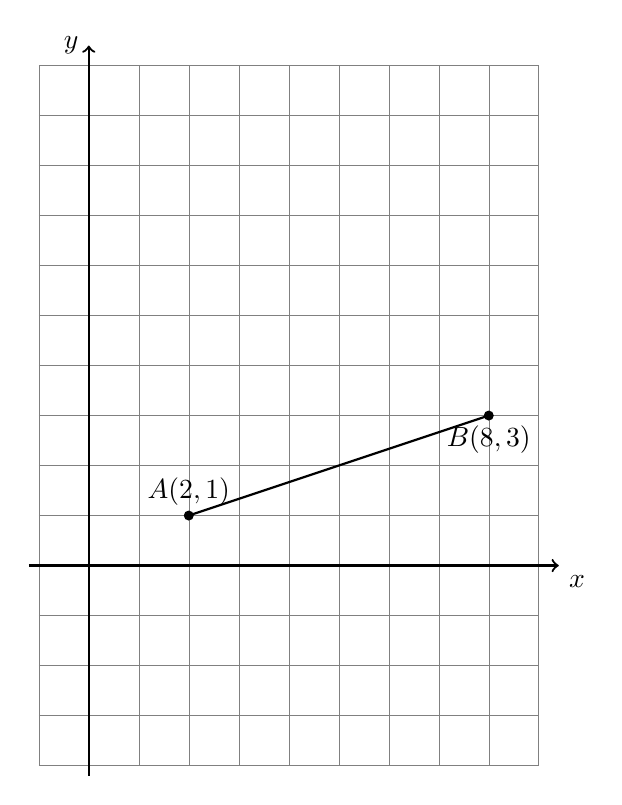
\begin{tikzpicture}[scale=.635]
      \draw [help lines] (-1,-4) grid (9,10);
      \draw [thick, ->] (-1.2,0) -- (9.4,0) node [below right] {$x$};
      \draw [thick, ->] (0,-4.2)--(0,10.4) node [left] {$y$};
      \draw [thick] (2,1)--(8,3);
      \fill (2,1) circle[radius=0.1cm]node[above]{$A(2,1)$};
      \fill (8,3) circle[radius=0.1cm]node[below ]{$B(8,3)$};
    \end{tikzpicture}
    \end{center} 
  \end{multicols}

\newpage

\item The line $l$ having the equation $\displaystyle y-2=-\frac{2}{3}(x-3)$ is shown below.
\begin{multicols}{2}
  \begin{enumerate}
    \item Write down coordinates of $P$.
    \item Point $P$ is mapped to the origin by\\ $x \rightarrow x-h$\\ $y \rightarrow y-k$ \\Write down $h$ and $k$.
    \item Plot the image of $l$ after the translation.
  \end{enumerate}
  \begin{flushright}
    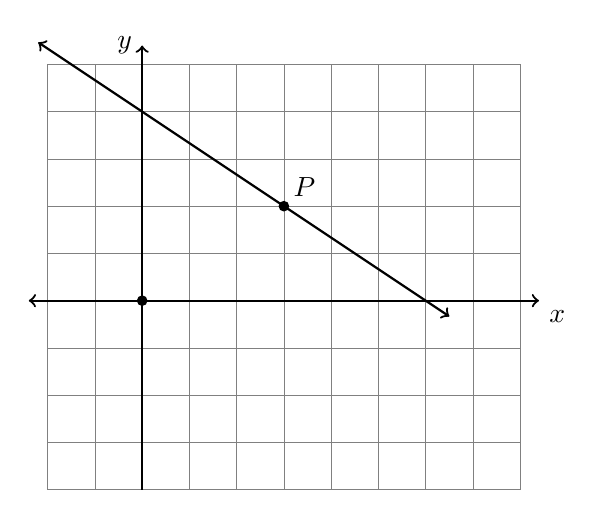
\begin{tikzpicture}[scale=0.6]
      \draw [help lines] (-2,-4) grid (8,5);
      \draw [thick, <->] (-2.4,0) -- (8.4,0) node [below right] {$x$};
      \draw [thick, ->] (0,-4.0)--(0,5.4) node [left] {$y$};
      \draw [thick,<->,samples=20,domain=-2.2:6.5] plot(\x,-2/3*\x+4);
      \draw [fill] (3,2) circle [radius=0.1] node[above right] {$P$};
      \draw [fill] (0,0) circle [radius=0.1];
    \end{tikzpicture}
  \end{flushright}
\end{multicols}%\vspace{1cm}

\item The function $f$ is plotted below for $x \ge 1$. Identify the equation represented by the graph.
\begin{multicols}{2}
  \begin{enumerate}
    \item $f(x) = \sqrt{x-1}+2$
  \end{enumerate}
\begin{center} 
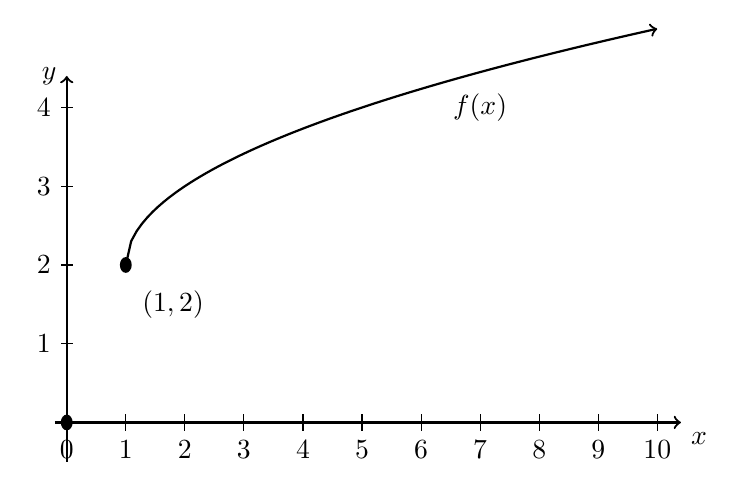
\begin{tikzpicture}[xscale=0.75, yscale=1]
  \draw [thick, ->] (-0.2,0) -- (10.4,0) node [below right] {$x$};
  \draw [thick, ->] (0,-0.5)--(0,4.4) node [left] {$y$};
  \foreach \x in {0,1,2,...,10} \draw (\x cm,3pt) -- (\x cm,-3pt) node[below] {$\x$};
  \foreach \y in {1,2,3,4} \draw (3pt,\y cm) -- (-3pt,\y cm) node[left] {$\y$};
  \fill (0,0) circle[radius=0.1];
  \draw [thick,->,samples=100,domain=1:10] plot(\x,{(\x-1)^0.5+2});
  \fill (1,2) circle[radius=0.1];
  \node at (1.8,1.5){$(1,2)$};
  \node at (7,4){$f(x)$};
\end{tikzpicture}
\end{center}
\end{multicols}


\item The function $g: y = |x-2|+3$ is plotted below as a solid line. What translation would map $g$ onto the parent function (dotted)?  State your answer in the form $x \rightarrow x-h$, $y \rightarrow y-k$.
\begin{center} 
\begin{tikzpicture}[xscale=1.0, yscale=1]
  \draw [thick, ->] (-5.2,0) -- (5.4,0) node [below right] {$x$};
  \draw [thick, ->] (0,-0.5)--(0,4.4) node [left] {$y$};
  \foreach \x in {-4,-3,-2,-1,1,2,3,4, 5} \draw (\x cm,3pt) -- (\x cm,-3pt) node[below] {$\x$};
  \foreach \y in {1,2,3,4} \draw (3pt,\y cm) -- (-3pt,\y cm) node[left] {$\y$};
  \draw [dashed,<->,samples=20,domain=-1.75:1.75] plot(\x,abs{\x});
  \fill (0,0) circle[radius=0.1];
  \draw [thick,<->,samples=50,domain=0:4] plot(\x,abs{(\x-2)}+3);
  \fill (2,3) circle[radius=0.1];
  \node at (2.5,2.5){$(2,3)$};
  \node at (4,4.5){$g(x)$};
\end{tikzpicture}
\end{center}

\item The line $\overleftrightarrow{RS}$ having the equation $\displaystyle y=\frac{2}{3}x+2$ is shown below.
\begin{multicols}{2}
  \begin{enumerate}
    \item Write down the slope of $\overleftrightarrow{RS}$,\\[0.25cm] $m=$
    \item Write down the $y$-intercept of $\overleftrightarrow{RS}$,\\[0.25cm] $b=$
    \item Dilate $\overleftrightarrow{RS}$ by a scale factor $k=2$ centered at the origin. Mark the images $R'$ and $S'$.
    \item Write down the equation of $\overleftrightarrow{R'S'}$
  \end{enumerate}
  \begin{flushright}
    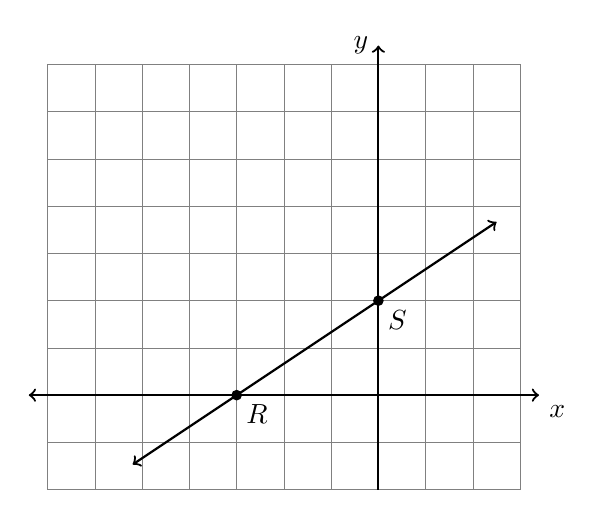
\begin{tikzpicture}[scale=0.6]
      \draw [help lines] (-7,-2) grid (3,7);
      \draw [thick, <->] (-7.4,0) -- (3.4,0) node [below right] {$x$};
      \draw [thick, ->] (0,-2.0)--(0,7.4) node [left] {$y$};
      \draw [thick,<->,samples=20,domain=-5.2:2.5] plot(\x,2/3*\x+2);
      \draw [fill] (-3,0) circle [radius=0.1] node[below right] {$R$};
      \draw [fill] (0,2) circle [radius=0.1] node[below right] {$S$};
    \end{tikzpicture}
  \end{flushright}
\end{multicols}%\vspace{1cm}

\item Complete the t-table for the parent function $f$: $y=x^2$, plot the points, and draw $f$ as a smooth curve.
  \begin{center} 
  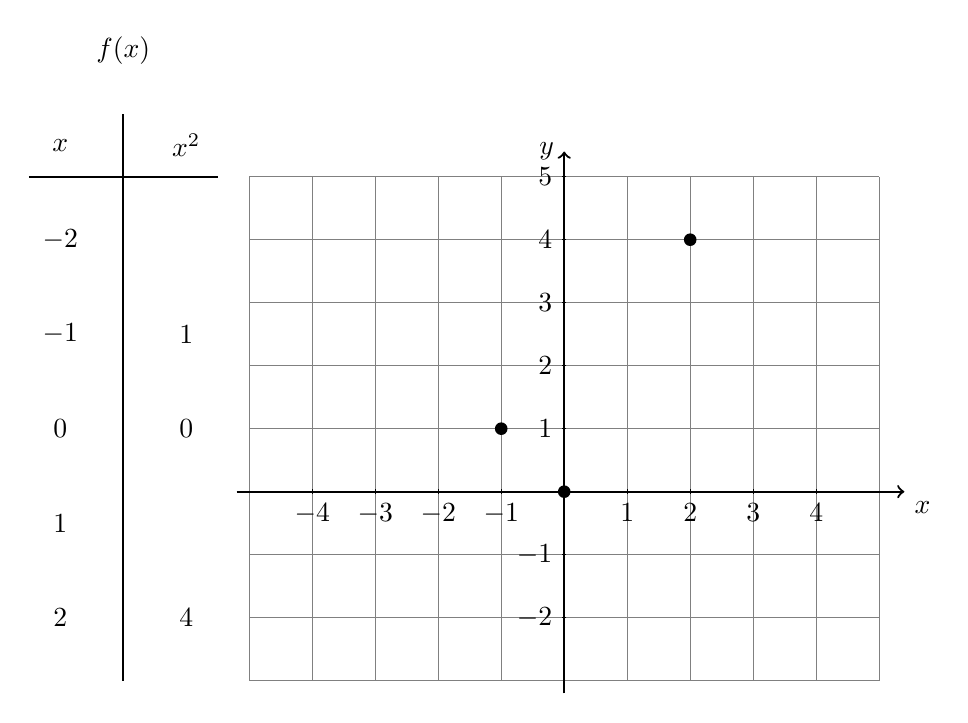
\begin{tikzpicture}[scale=0.8]
    \draw [help lines] (-5,-3) grid (5,5);
    \draw [thick, ->] (-5.2,0) -- (5.4,0) node [below right] {$x$};
    \draw [thick, ->] (0,-3.2)--(0,5.4) node [left] {$y$};
    \foreach \x in {-4,-3,-2,-1,1,2,3,4} \draw (\x cm,1pt) -- (\x cm,-1pt) node[below] {$\x$};
    \foreach \y in {-2,-1,1,2,3,4,5} \draw (1pt,\y cm) -- (-1pt,\y cm) node[anchor=east] {$\y$};
    \draw [thick] (-7,-3) -- (-7,6);
    \draw [thick] (-8.5,5) -- (-5.5,5);
    \node at (-7,7){$f(x)$};
    \node at (-8,5.5){$x$}; \node at (-6,5.5){$x^2$};
    \node at (-8,4){$-2$};
    \node at (-8,2.5){$-1$}; \node at (-6,2.5){$1$};
    \node at (-8,1){$0$};  \node at (-6,1){$0$};
    \node at (-8,-0.5){$1$};
    \node at (-8,-2){$2$}; \node at (-6,-2){$4$};
    %\fill (-2,4) circle[radius=0.1];
    \fill (-1,1) circle[radius=0.1];
    \fill (0,0) circle[radius=0.1];
    %\fill (1,1) circle[radius=0.1];
    \fill (2,4) circle[radius=0.1];
  \end{tikzpicture}
  \end{center}

  \item Write down the translation that would map $g(x)$ onto the parent function $y=x^2$. State your answer in the form $x \rightarrow x-h$, $y \rightarrow y-k$.
  \begin{center} 
  \begin{tikzpicture}[xscale=1, yscale=1]
    \draw [thick, ->] (-5.2,0) -- (5.4,0) node [below right] {$x$};
    \draw [thick, ->] (0,-0.5)--(0,4.4) node [left] {$y$};
    \foreach \x in {-4,-3,-2,-1,1,2,3,4, 5} \draw (\x cm,3pt)--(\x cm,-3pt) node[below] {$\x$};
    \foreach \y in {1,2,3,4} \draw (3pt,\y cm)--(-3pt,\y cm) node[left] {$\y$};
    \draw [dashed,<->,samples=20,domain=-1.75:1.75] plot(\x,\x*\x);
    \fill (0,0) circle[radius=0.1];
    \draw [thick,<->,samples=20,domain=3.25:6.75] plot(\x,{(\x-5)^2+1});
    \fill (5,1) circle[radius=0.1];
    \node at (5.5,0.5){$(5,1)$};
    \node at (4,3.5){$g(x)$};
  \end{tikzpicture}
  \end{center}

\item The parabola $y+1=(x-2)^2$ graphed below.
  \begin{multicols}{2}
  \begin{enumerate}
    \item Write down its $y$-intercept.
    \item Write down its $x$-intercepts.
    \item Reflect $f$ across the $y$-axis.
    \item Mark and label the image\\ parabola's intercepts and vertex.
  \end{enumerate}
  \begin{center} 
  \begin{tikzpicture}[xscale=1, yscale=1]
    \draw [thick, ->] (-3.2,0) -- (5.4,0) node [above left] {$x$};
    \draw [thick, ->] (0,-0.5)--(0,4.4) node [left] {$y$};
    \foreach \x in {-3,-2,-1,1,2,3,4, 5} \draw (\x cm,3pt)--(\x cm,-3pt) node[below] {$\x$};
    \foreach \y in {1,2,3} \draw (3pt,\y cm)--(-3pt,\y cm) node[left] {$\y$};
    \draw [thick,<->,samples=40,domain=-0.25:4.25] plot(\x,{(\x-2)^2-1});
    \fill (2,-1) circle[radius=0.08];
    \node at (2.5,-1.5){$(2,-1)$};
    \node at (4.5,3){$f(x)$};
  \end{tikzpicture}
  \end{center}
  \end{multicols}

\item Part of the exponential function $f$: $y=x^2$, is shown below. 
  \begin{multicols}{2}
    \begin{enumerate}
      \item Reflect $f$ across the $x$-axis.
      \item Write down the coordinates of $P$.
      \item Mark and label the image $P'$ with its coordinates. \vspace{2cm}
    \end{enumerate}
    \begin{flushright}
      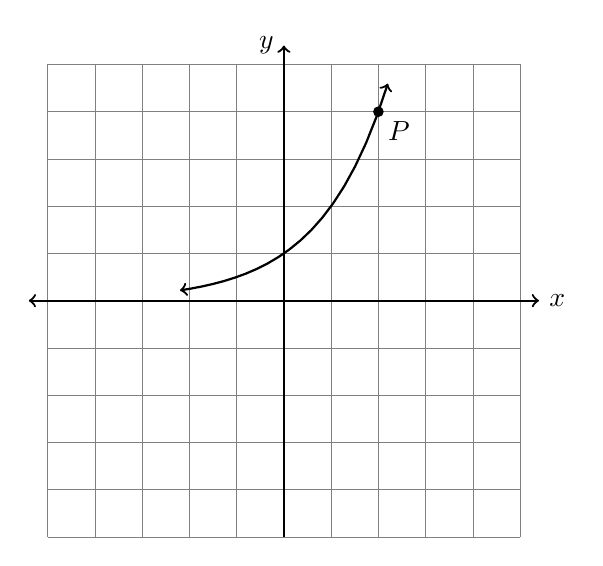
\begin{tikzpicture}[scale=0.6]
      \draw [help lines] (-5,-5) grid (5,5);
      \draw [thick, <->] (-5.4,0) -- (5.4,0) node [right] {$x$};
      \draw [thick, ->] (0,-5)--(0,5.4) node [left] {$y$};  
      \draw [thick,<->,samples=20,domain=-2.2:2.2] plot(\x,2^\x);
      \draw [fill] (2,4) circle [radius=0.1] node[below right] {$P$};
    \end{tikzpicture}
  \end{flushright}
  \end{multicols}

\item The function $f$ is plotted below for $x \ge 1$. Identify the equation represented by the graph. (normal function)
\begin{multicols}{2}
  \begin{enumerate}
    \item $f(x) = \sqrt{x-1}+2$
    \item The Normal distribution $N(\mu, \sigma)$
    \item Reciprocal function $\displaystyle y=\frac{1}{x}$
  \end{enumerate}
\begin{center} 
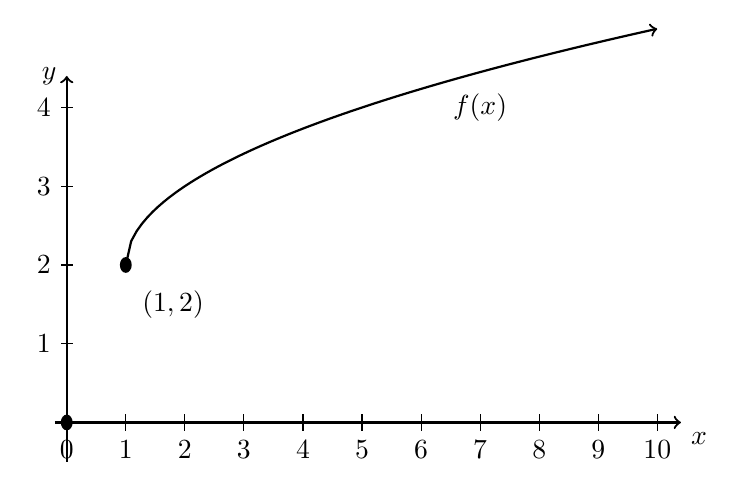
\begin{tikzpicture}[xscale=0.75, yscale=1]
  \draw [thick, ->] (-0.2,0) -- (10.4,0) node [below right] {$x$};
  \draw [thick, ->] (0,-0.5)--(0,4.4) node [left] {$y$};
  \foreach \x in {0,1,2,...,10} \draw (\x cm,3pt) -- (\x cm,-3pt) node[below] {$\x$};
  \foreach \y in {1,2,3,4} \draw (3pt,\y cm) -- (-3pt,\y cm) node[left] {$\y$};
  \fill (0,0) circle[radius=0.1];
  \draw [thick,->,samples=100,domain=1:10] plot(\x,{(\x-1)^0.5+2});
  \fill (1,2) circle[radius=0.1];
  \node at (1.8,1.5){$(1,2)$};
  \node at (7,4){$f(x)$};
\end{tikzpicture}
\end{center}
\end{multicols}


\item The circle with center $P$ shown below can be represented by an equation of the form $(x-h)^2+(y-k)^2=r^2$. 
  \begin{multicols}{2}
    \begin{enumerate}
      \item Reflect $f$ across the $x$-axis.
      \item Write down the radius of circle $P$.
      \item Mark and label the image $P'$ with its coordinates. \vspace{2cm}
    \end{enumerate}
    \begin{flushright}
      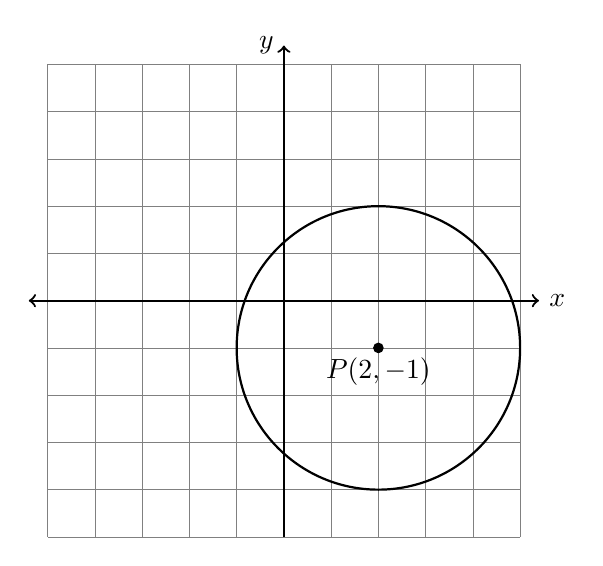
\begin{tikzpicture}[scale=0.6]
      \draw [help lines] (-5,-5) grid (5,5);
      \draw [thick, <->] (-5.4,0) -- (5.4,0) node [right] {$x$};
      \draw [thick, ->] (0,-5)--(0,5.4) node [left] {$y$};  
      \draw [thick] (2,-1) circle[radius=3];
      \draw [fill] (2,-1) circle [radius=0.1] node[below] {$P(2,-1)$};
    \end{tikzpicture}
  \end{flushright}
  \end{multicols}

\item The reciprocal function shown below has the equation $\displaystyle f(x) =\frac{1}{x-1}-2$. Its asymptotes are plotted as dotted lines.
\begin{multicols}{2}
  \begin{enumerate}
    \item Write down the equation of the horizontal asymptote. \vspace{2cm}
    \item Write down the equation of the vertical asymptote.
  \end{enumerate}
  \begin{flushright}
    \begin{tikzpicture}
      \draw [thick, <->] (-3.4,0) -- (3.4,0) node [right] {$x$};
      \draw [thick, ->] (0,-2.5)--(0,2.4) node [left] {$y$};  
      \draw [thick,<->,samples=20,domain=-3.2:-0.5] plot(\x,1/\x);
      \draw [thick,<->,samples=20,domain=0.4:3.2] plot(\x,1/\x);
      \draw [thick] (1,3) circle[radius=0.1];
    \end{tikzpicture}
\end{flushright}
\end{multicols}

\item The sine function in the graph has the form $f(x)=k \sin x + b$, where the parameter $b$ is the vertical translation and the coefficient $k$ is the vertical stretch factor. $f$ passes through the points $(90^\circ, 3)$ and $(270^\circ, -1)$. Write down the parameter values:
\begin{multicols}{2}
  \begin{enumerate}
    \item $b=$ \vspace{1cm}
    \item $k=$
  \end{enumerate}\vspace{1cm}
  \begin{center}
    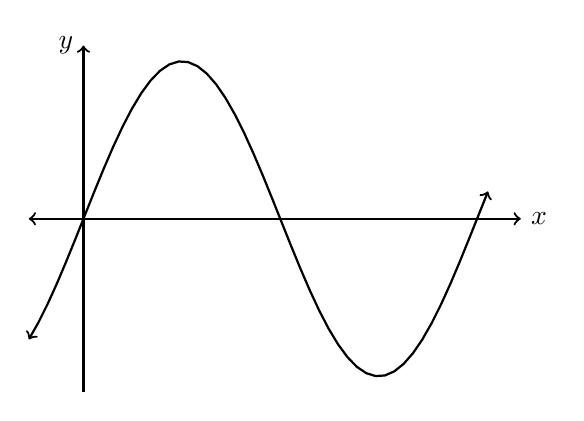
\begin{tikzpicture}[xscale=5/360, yscale=2]
      \draw [thick, <->] (-50,0) -- (400,0) node [right] {$x$};
      \draw [thick, ->] (0,-1.1)--(0,1.1) node [left] {$y$};  
      \draw [thick,<->,samples=50,domain=-50:370] plot(\x,{sin(\x)});
    \end{tikzpicture}
  \end{center}
\end{multicols}

\end{enumerate}
\end{document}
